\documentclass[a4paper]{article}

%% Language and font encodings
\usepackage{CJKutf8}
\usepackage[english]{babel}
\usepackage[T1]{fontenc}

%% Sets page size and margins
\usepackage[a4paper,top=3cm,bottom=2cm,left=3cm,right=3cm,marginparwidth=1.75cm]{geometry}

%% Useful packages
\usepackage{amsmath}
\usepackage{graphicx}
\usepackage[colorinlistoftodos]{todonotes}
\usepackage[colorlinks=true, allcolors=blue]{hyperref}
\usepackage{enumitem}

\title{Assignment01. About the utility git}

\author{중앙대학교 컴퓨터공학부 \\20120115 조한솔}

\begin{document}
\begin{CJK}{UTF8}{mj}
\maketitle

\begin{abstract}
CAU Mathematical Foundations for
Computer Vision and Machine Learning Assignment01
\end{abstract}

\section{Contents}

\begin{enumerate}
\item Basic Usage
\item Conventions
\item Comand in Detail
	\begin{enumerate}[label=(\alph*)]
    \item Diff
    \item Commit
    \item Checkout
    \item Committing with a Detached HEAD
    \item Reset
    \item Merge
    \item Cherry Pick
    \item Rebase
    \end{enumerate}
\item Screenshot of the project at GitHub
\end{enumerate}

%
% Basic Usage
%
\section{Basic Usage}

The four commands above copy files between the working directory, the stage (also called the index), and the history (in the form of commits).

\begin{itemize}
\item git add files copies files (at their current state) to the stage,
\item git commit saves a snapshot of the stage as a commit,
\item git reset -- files unstages files; that is, it copies files from the latest commit to the stage.\\Use this command to "undo" a git add files. You can also git reset to unstage everything,
\item git checkout -- files copies files from the stage to the working directory. Use this to throw away local changes.

\end{itemize}
You can use git reset -p, git checkout -p, or git add -p instead of (or in addition to) specifying particular files to interactively choose which hunks copy.
It is also possible to jump over the stage and check out files directly from the history or commit files without staging first.

\begin{itemize}
\item git commit -a is equivalent to running git add on all filenames that existed in the latest commit, and then running git commit,
\item git commit files creates a new commit containing the contents of the latest commit, plus a snapshot of files taken from the working directory. Additionally, files are copied to the stage,
\item git checkout HEAD -- files copies files from the latest commit to both the stage and the working directory.
\end{itemize}
\pagebreak

\subsection{Conventions}


In the rest of this document, we will use graphs of the following form.

\begin{center}
\centering
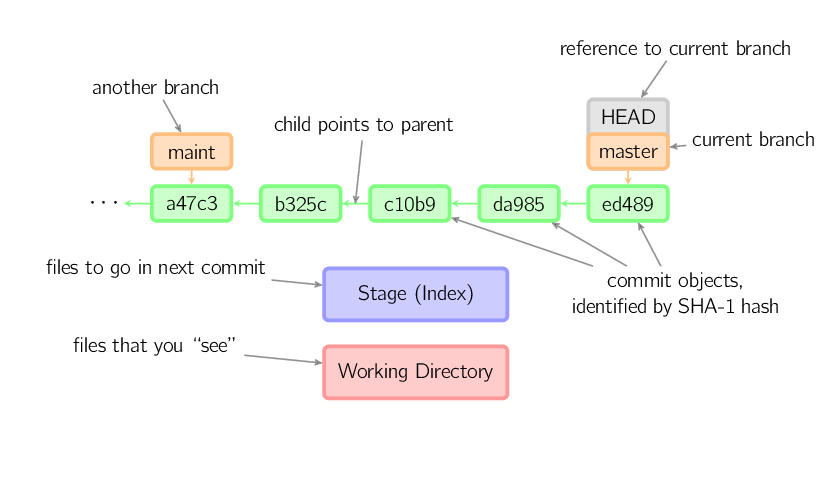
\includegraphics[width=1\textwidth]{conventions.png}
\end{center}
Commits are shown in green as 5-character IDs, and they point to their parents. Branches are shown in orange, and they point to particular commits. The current branch is identified by the special reference HEAD, which is "attached" to that branch. In this image, the five latest commits are shown, with ed489 being the most recent. master (the current branch) points to this commit, while maint (another branch) points to an ancestor of master's commit.

\subsection{Commands in Detail}

\begin{enumerate}[label=(\alph*)]
\item Diff

There are various ways to look at differences between commits. Below are some common examples. Any of these commands can optionally take extra filename arguments that limit the differences to the named files.

\item Commit

When you commit, git creates a new commit object using the files from the stage and sets the parent to the current commit. It then points the current branch to this new commit. In the image below, the current branch is master. Before the command was run, master pointed to ed489. Afterward, a new commit, f0cec, was created, with parent ed489, and then master was moved to the new commit.

\item Checkout

The checkout command is used to copy files from the history (or stage) to the working directory, and to optionally switch branches.

When a filename (and/or -p) is given, git copies those files from the given commit to the stage and the working directory. For example, git checkout HEAD~ foo.c copies the file foo.c from the commit called HEAD~ (the parent of the current commit) to the working directory, and also stages it. (If no commit name is given, files are copied from the stage.) Note that the current branch is not changed.
\newpage
\item Committing with a Detached HEAD

When HEAD is detached, commits work like normal, except no named branch gets updated. (You can think of this as an anonymous branch.)
Once you check out something else, say master, the commit is (presumably) no longer referenced by anything else, and gets lost. Note that after the command, there is nothing referencing 2eecb.
If, on the other hand, you want to save this state, you can create a new named branch using git checkout -b name.

\item Reset

The reset command moves the current branch to another position, and optionally updates the stage and the working directory. It also is used to copy files from the history to the stage without touching the working directory.

If a commit is given with no filenames, the current branch is moved to that commit, and then the stage is updated to match this commit. If --hard is given, the working directory is also updated. If --soft is given, neither is updated.

\item Merge

A merge creates a new commit that incorporates changes from other commits. Before merging, the stage must match the current commit. The trivial case is if the other commit is an ancestor of the current commit, in which case nothing is done. The next most simple is if the current commit is an ancestor of the other commit. This results in a fast-forward merge. The reference is simply moved, and then the new commit is checked out.

\item Cherry Pick

The cherry-pick command "copies" a commit, creating a new commit on the current branch with the same message and patch as another commit.

\item Rebase

A rebase is an alternative to a merge for combining multiple branches. Whereas a merge creates a single commit with two parents, leaving a non-linear history, a rebase replays the commits from the current branch onto another, leaving a linear history. In essence, this is an automated way of performing several \textcolor{red}{cherry-picks} in a row.

\end{enumerate}



\subsection{Screenshot of the project at GitHub}

\begin{figure}[h!]
	\centering
	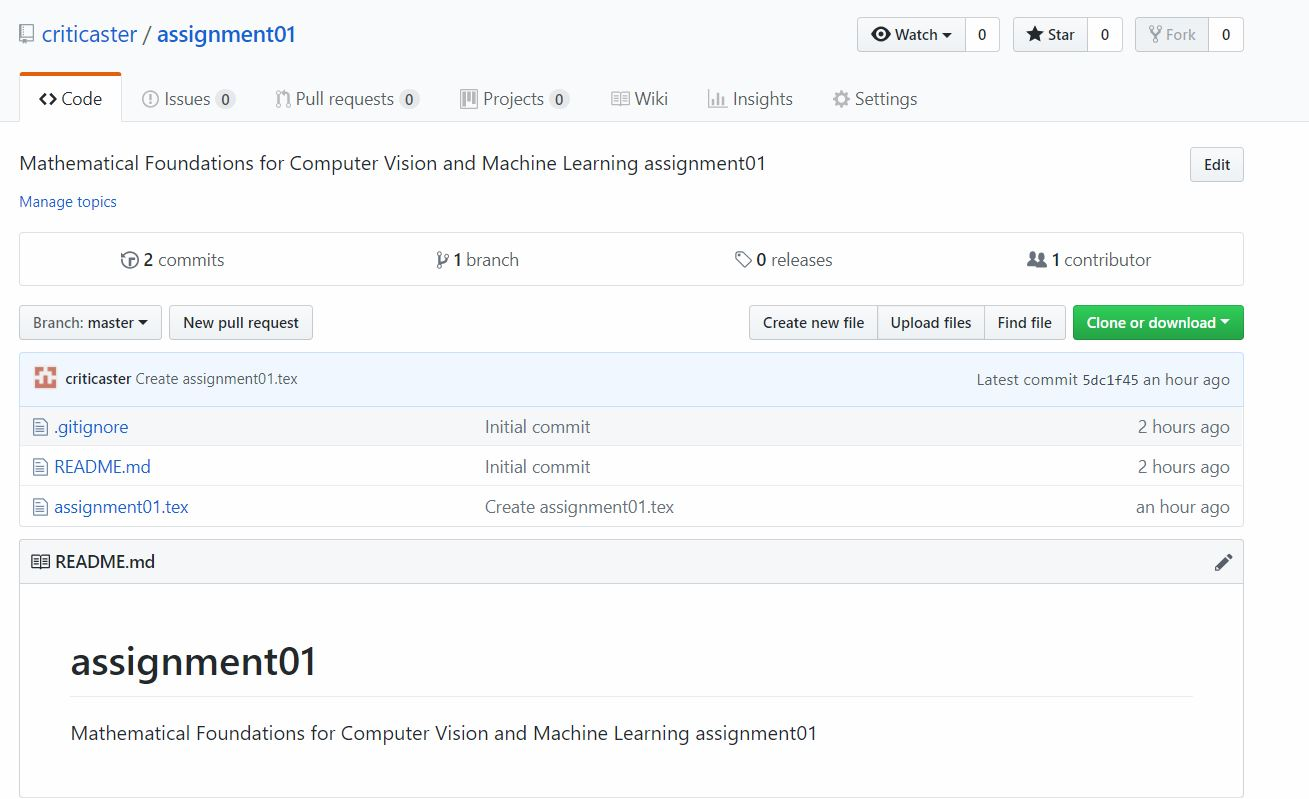
\includegraphics[width=0.8\textwidth]{ag01}
	\caption{Screenshot of the project at GitHub}
\end{figure}

Link : \href{https://github.com/criticaster/assignment01}
    {https://github.com/criticaster/assignment01}

\end{CJK}
\end{document}